%% Submission to Automated Software Engineering (Springer), Springer Nature LaTeX template (author-year references).
%% Tables in tables/ are generated by make_tables.mjs.
\documentclass[pdflatex,sn-basic]{sn-jnl}

\usepackage{graphicx}
\usepackage{multirow}
\usepackage{amsmath,amssymb}
\usepackage{booktabs}
\usepackage{array}
\usepackage{tikz}
\usetikzlibrary{positioning,arrows.meta}
\usepackage{xcolor}
\usepackage{xurl}
\def\burl#1{\url{#1}}

\begin{document}

\title[Executable oracles as acceptance gates for LLM-generated simulators]{Where and What: Executable Oracles as Acceptance Gates and Repair Feedback for LLM-Generated Mechanism Simulators}

\author*[1]{\fnm{Hai} \sur{Hoang}}\email{haihpaws@gmail.com}
\affil*[1]{\orgdiv{FPT School of Business and Technology (FSB)}, \orgname{FPT University}, \orgaddress{\city{Ho Chi Minh City}, \country{Vietnam}}}

%% Journal guide: 150-250 words, no undefined abbreviations, no citations. Current count: see wc.
\abstract{Large language models can write interactive 3D simulators of machines from short descriptions. Such programs run and look plausible, yet they can be kinematically wrong, and current pipelines accept them after a vision-language model has looked at screenshots. We present an executable test oracle for generated mechanism simulators. It samples the page's pure rendering function over time and checks structural invariants, the dimensions the simulator declares, engineering design rules, and the kinematic solution computed from those declared dimensions without per-task specifications. Using eight mechanisms, 88 simulators from two models of one vendor (plus 20 from another vendor), we ask which errors occur, what the oracle and a vision-language reviewer detect, whether the oracle can gate iterative repair, and how specific its feedback must be. Under free-form specifications, 20 of 80 simulators were wrong, mostly in design knowledge such as misassigned published link lengths; visual review missed invisible faults such as an impossible gear assembly. In repair of at most three rounds, feedback naming the faulty element with its correct value fixed 28 of 28 faulty cases; naming the element only, 15 of 28; naming the failed check and its magnitude, 11 of 28; self-refinement without feedback, 7 of 28; and the visual reviewer in the loop, 5 of 22. The information needed depends on the repairing model: on design-knowledge errors the smaller model succeeded only when given the correct value (13 of 13 versus 0 of 13), while the larger one needed only the location (7 of 7).}


\keywords{test oracle, LLM code generation, automated program repair, simulation verification and validation, metamorphic testing, vision-language models}

\maketitle

\section{Introduction}\label{sec:intro}

Large language models (LLMs) are increasingly used to produce not only snippets of code but complete, runnable artefacts: interactive scientific demonstrations \cite{chen2025interactscience}, physics animations \cite{wang2026simuscene,shende2026perceptual}, articulated 3D objects \cite{gao2026lam,le2025articulate}, CAD models \cite{alrashedy2025cad} and whole 3D worlds \cite{lu2026worldcoder}. One instance of this trend is the \emph{mechanism simulator}: a single web page in which a machine (a linkage, a gear train, a cam, a walking leg) is drawn in 3D and moves, with live numbers that explain it. Tools that generate such pages from a one-paragraph request are already available to end users \cite{teardown}. They are attractive for engineering education, design communication and, increasingly, as lightweight digital twins.

Such a page has a peculiar correctness problem. It almost always loads and animates, and it usually looks right. Whether it is \emph{kinematically} right---whether the parts stay connected, follow the motion the machine actually has, and respect the design rules that make the machine work---cannot be seen in a handful of frames and is not covered by any unit test, because there are none. In the generation pipelines we are aware of, the acceptance step is a vision-language model (VLM) that inspects screenshots \cite{shende2026perceptual,le2025articulate,alrashedy2025cad}. This is a mechanised version of the oldest simulation-validation technique, watching the animation \cite{sargent2013vv}, with the same weakness: plausible-looking motion is accepted.

Consider Theo Jansen's walking leg \cite{jansen_strandbeest}. Its eleven link lengths, the ``holy numbers'', make the foot trace a path with a long flat bottom. In our study, both models we tested remembered the eleven numbers but often assigned them to the wrong links. The resulting legs assemble, move smoothly and look like Jansen legs, but the flat stride shrinks from about a third of the cycle to a few percent. A VLM shown the frames reported the leg as correct in some runs and as faulty in others. When asked to re-check its own work, the generating model asserted that the lengths ``match the published holy numbers'' and, when told otherwise, that the checker must be wrong. An executable check that compares the declared lengths with the published ones settles the question in a fraction of a second and can also say which link is wrong and what its length should be.

This paper studies such executable oracles for LLM-generated mechanism simulators, both as an \emph{acceptance gate} and as a source of \emph{repair feedback}. The oracle (Section~\ref{sec:approach}) needs no hand-written specification per task. A minimal output contract asks the generator to expose a pure function \texttt{render(t)}, the dimensions it chose, and named marker points on each part. From these, the oracle derives metamorphic and structural checks (determinism under reordered calls, periodicity, rigid parts, coincident joints), checks the drawing against the declared dimensions, applies engineering design rules, and compares every marker with the kinematic solution computed from the declared dimensions. When a check fails, it reports where (which link, joint or marker, at which instant) and, where a ground truth exists, what the value should be.

We address four research questions:
\begin{itemize}
\item \textbf{RQ1} Which errors do LLMs make when generating mechanism simulators from free-form descriptions, and how often?
\item \textbf{RQ2} Which errors do the oracle and a VLM reviewer detect?
\item \textbf{RQ3} Does the oracle work as an acceptance gate for iterative repair, compared with VLM review in the loop and self-refinement?
\item \textbf{RQ4} How specific must the oracle's feedback be, and does the answer depend on the repairing model?
\end{itemize}

We study eight mechanisms, 88 generated simulators, 39 seeded mutants and nearly 300 repair attempts by two models of different size from the same family. The main findings are:
\begin{itemize}
\item Free-form specifications lead to errors in 20 of 80 simulators; detailed specifications lead to none in 8. Errors concentrate in design knowledge that must be recalled (Jansen's link lengths, Chebyshev's lambda proportions) and in assembly conditions. Mechanisms whose design rule can be stated as a relation (a cam's motion law, the Peaucellier--Lipkin conditions) produced no errors.
\item The oracle and the VLM catch different error classes. The oracle catches design-knowledge and invisible errors; the VLM catches geometry outside the oracle's contract. The VLM's detection of length errors depends largely on reading the numeric panel.
\item As a repair gate, oracle feedback that names the faulty element and its correct value fixes 28 of 28 faulty file-runs within two rounds. VLM review in the loop fixes 5 of 22 and self-refinement 7 of 28. VLM-driven loops stop early on wrong ``correct'' verdicts.
\item Specificity matters in a model-dependent way. On design-knowledge errors, the smaller model succeeded only with the correct value (13/13 versus 0/13 with location only). The larger model needed only the location (7/7) (Fisher's exact test, $p = 1.3\times10^{-5}$).
\end{itemize}

The contributions are: (i) an executable oracle for generated mechanism simulators that needs no per-task specification and includes a guard against marker gaming; (ii) a controlled comparison of oracle, VLM and self-refinement feedback in iterative repair with oracle-gated stopping; (iii) a feedback-specificity ablation showing an interaction between the information content of feedback and the repairing model; and (iv) the full dataset of specifications, generated and repaired simulators, mutants and oracle reports, available at \url{https://github.com/haihpse150218/llm-mechsim-oracle}.

Beyond education, the questions matter wherever simulation software is produced quickly and trusted on sight. This includes digital twins, operator training and design reviews, which are the kinds of systems in which NASA and other mission-critical organisations rely on simulation V\&V \cite{sargent2013vv,balci1997vva}. An acceptance gate that is cheap, deterministic and explains its verdict is a natural complement to human or model-based visual review.

Section~\ref{sec:background} gives background, Section~\ref{sec:approach} describes the oracle, Section~\ref{sec:design} the study design, Section~\ref{sec:results} the results, Section~\ref{sec:discussion} discusses them, Section~\ref{sec:threats} covers threats to validity, Section~\ref{sec:related} related work, and Section~\ref{sec:conclusion} concludes.

\section{Background}\label{sec:background}

\subsection{Test oracles and derived oracles}
A test oracle decides whether an observed behaviour is correct \cite{barr2015oracle}. Barr et al.\ distinguish specified oracles (from a formal specification), derived oracles (from other artefacts such as documentation, earlier versions or properties of the program), implicit oracles (crashes, exceptions) and human oracles. Metamorphic testing \cite{chen2018metamorphic,segura2016survey} is the best-known family of derived oracles: instead of the correct output for one input, it checks a relation between outputs of related executions. Metamorphic and differential oracles are well established for scientific software \cite{kanewala2014scientific}, autonomous-driving software \cite{zhou2019driverless} and graphics drivers \cite{donaldson2017shader}, where exact expected outputs are unavailable. Recent work generates oracles or assertions with neural models \cite{dinella2022toga,hossain2023neural} and discusses the risks of letting an LLM act as the oracle for code that an LLM wrote \cite{molina2025oracle}. For LLM-generated code in particular, weak test suites accept many incorrect programs \cite{liu2023evalplus}.

\subsection{Kinematics of planar mechanisms}
All mechanisms in this study are planar and driven by a single input, a crank turning or swinging at constant angular speed. The position of every joint follows from the input angle by solving loop-closure equations. For the linkages used here, each unknown joint is the intersection of two circles centred on joints already known. Each intersection has two solutions, the \emph{assembly branches}, and a correct simulator must stay on one branch throughout the cycle. Whether a solution exists for every input angle (the linkage \emph{assembles}) depends on the link lengths. The Grashof condition, for example, decides whether a four-bar's crank can turn fully. Beyond assembly, many mechanisms work only because of specific \emph{design knowledge}:
\begin{itemize}
\item \emph{published dimensions}, such as Jansen's eleven link lengths \cite{jansen_strandbeest} or the proportions of Chebyshev's lambda linkage, crank $a$, ground $2a$, rocker $2.5a$, coupler $2.5a$ extended by a further $2.5a$ to the tracing point \cite{wiki_lambda};
\item \emph{relations}, such as the Peaucellier--Lipkin conditions (equal rhombus sides, equal long arms, crank length equal to the distance between the fixed pivots), under which the output point moves on an exact straight line;
\item \emph{assembly conditions}, such as the requirement that the sum of sun and ring teeth of a planetary set be divisible by the number of equally spaced planets.
\end{itemize}
Errors in design knowledge are particularly treacherous. The mechanism still assembles and moves smoothly, but it does not do what it is for.

\subsection{Generated simulators and their acceptance}
We consider simulators written as one self-contained HTML page using \texttt{three.js}, as produced by the \emph{teardown} skill for Claude Code \cite{teardown}. The skill's own review loop has the model look at sheets of rendered frames and correct what it sees. The same pattern appears in research systems that use a VLM as critic of generated 3D or physics code \cite{le2025articulate,alrashedy2025cad,shende2026perceptual,gao2026lam}. In the terms of simulation V\&V \cite{sargent2013vv,balci1997vva}, this is the \emph{animation} technique: watching the model run to judge its behaviour. It is useful for gross errors, but it cannot reveal quantities that are not visible and is prone to rationalising small discrepancies. The comparison of a model's output with an analytic solution, the other classical technique, has so far not been applied to generated simulators. Making it possible requires access to the simulator's internal state at arbitrary times, which motivates the minimal output contract of Section~\ref{sec:approach}.

\section{An executable oracle for generated mechanism simulators}\label{sec:approach}

\subsection{Output contract}
The generator receives a short prose description of the mechanism, for example ``one leg of Theo Jansen's Strandbeest walking linkage, with the link lengths of Jansen's published holy numbers'', together with a fixed output contract. It chooses all dimensions, placement, speed and direction itself. The contract asks for:
\begin{enumerate}
\item one self-contained HTML page that loads \texttt{three.js} from a fixed path and no other network resource;
\item one named \texttt{Object3D} per listed part (for example \texttt{crank}, \texttt{coupler}, \texttt{rocker}), holding all of that part's meshes, and a child marker named \texttt{<part>@<point>} at each listed joint of that part (\texttt{crank@A}, \texttt{coupler@A}, \ldots);
\item a panel element per listed quantity, marked with a \texttt{data-q} attribute (for example the crank angle and the foot position);
\item an object \texttt{window.SIM} exposing the scene, the period, the parameters the simulator actually uses (\texttt{SIM.params}: link lengths, pivot positions, angular speed, initial angle) and a function \texttt{render(t)} that poses all parts and the panel for time $t$. The function must be \emph{pure}: no randomness, no clock, no state carried between calls.
\end{enumerate}
The contract fixes \emph{names}, not dimensions. It is a reduced version of the teardown skill's own contract \cite{teardown}, which already requires a pure \texttt{render(t)} so that videos can be captured frame by frame. In a first phase we also tried a detailed specification that fixed coordinate frames, assembly branches and formulas; it is discussed in Section~\ref{sec:design}.

\subsection{Sampling}
The oracle loads the page in headless Chrome through Playwright and waits for a readiness flag. It then calls \texttt{render(t)} at 120 instants per input period (two periods for the Geneva drive) and records the world position of every marker and the text of every panel element. Times are offset by a small irrational fraction of the period to avoid special angles. Tolerances scale with the machine: lengths are compared to within 1~mm per 100~mm of machine size (at least 1~mm), angles to within $1^\circ$, and relative quantities to within 1\%.

\subsection{Check families}
Figure~\ref{fig:oracle} gives an overview and Table~\ref{tab:checks} lists the checks. They fall into five families, ordered by how much ground truth they need.

%% Figure: the executable oracle (single column). Requires tikz with positioning, arrows.meta, fit.
\begin{figure}[t]
\centering
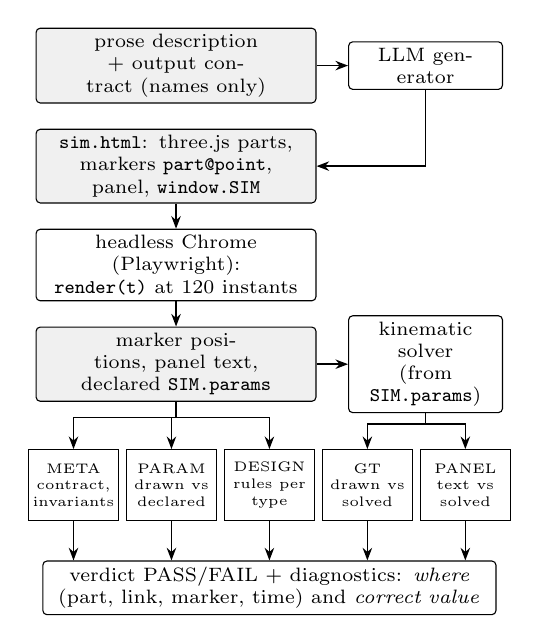
\begin{tikzpicture}[
  font=\scriptsize, node distance=3.2mm,
  box/.style={draw, rounded corners=1.5pt, align=center, inner sep=2.2pt, minimum height=6mm},
  data/.style={box, fill=black!6},
  fam/.style={draw, align=center, inner sep=1.6pt, minimum width=11.5mm, minimum height=9mm, font=\tiny},
  arr/.style={-{Stealth[length=1.6mm]}, semithick}]
\node[data, text width=34mm] (spec) {prose description\\ + output contract (names only)};
\node[box, right=4mm of spec, text width=18mm] (llm) {LLM generator};
\node[data, below=of spec, text width=34mm] (sim) {\texttt{sim.html}: three.js parts, markers \texttt{part@point}, panel, \texttt{window.SIM}};
\node[box, below=of sim, text width=34mm] (pw) {headless Chrome (Playwright):\\ \texttt{render(t)} at 120 instants};
\node[data, below=of pw, text width=34mm] (obs) {marker positions, panel text,\\ declared \texttt{SIM.params}};
\node[box, right=4mm of obs, text width=18mm] (solve) {kinematic solver\\ (from \texttt{SIM.params})};
\node[fam, below=6mm of obs.south west, anchor=north west, xshift=-1mm] (meta) {META\\ contract,\\ invariants};
\node[fam, right=0.8mm of meta] (param) {PARAM\\ drawn vs\\ declared};
\node[fam, right=0.8mm of param] (design) {DESIGN\\ rules per\\ type};
\node[fam, right=0.8mm of design] (gt) {GT\\ drawn vs\\ solved};
\node[fam, right=0.8mm of gt] (panel) {PANEL\\ text vs\\ solved};
\node[box, below=5mm of design, text width=56mm] (out) {verdict PASS/FAIL + diagnostics: \emph{where} (part, link, marker, time) and \emph{correct value}};
\draw[arr] (spec) -- (llm);
\draw[arr] (llm) |- (sim);
\draw[arr] (sim) -- (pw);
\draw[arr] (pw) -- (obs);
\draw[arr] (obs) -- (solve);
\draw[arr] (obs.south) -- ++(0,-2mm) -| (meta.north);
\draw[arr] (obs.south) -- ++(0,-2mm) -| (param.north);
\draw[arr] (obs.south) -- ++(0,-2mm) -| (design.north);
\draw[arr] (solve.south) -- ++(0,-1.4mm) -| (gt.north);
\draw[arr] (solve.south) -- ++(0,-1.4mm) -| (panel.north);
\foreach \f in {meta,param,design,gt,panel} \draw[arr] (\f.south) -- (\f.south |- out.north);
\end{tikzpicture}
\caption{The executable oracle. The generator chooses all dimensions; the oracle samples the page's pure \texttt{render(t)}, compares what is drawn with what the page declares, applies per-type design rules, and solves the kinematics from the declared parameters, so no per-task reference is written by hand.}\label{fig:oracle}
\end{figure}


\begin{table*}[t]
\caption{Check families of the oracle. Only DESIGN encodes mechanism-specific engineering knowledge; GT and PANEL use the kinematic solution computed from the simulator's own declared parameters.}\label{tab:checks}
\begin{tabular*}{\textwidth}{@{\extracolsep\fill}lp{0.38\textwidth}p{0.42\textwidth}}
\toprule
Family & Checks & Ground truth needed \\
\midrule
META & determinism under reversed call order; periodicity ($t$ vs.\ $t+T$); rigidity of every part (marker distances constant); coincidence of every shared joint; fixed frame static; markers rigidly attached to their part's geometry (drift) & none (metamorphic and structural relations implied by the contract) \\
PARAM & drawn distances between markers equal the declared link lengths; fixed pivots at declared positions; input angle equals $\theta_0+\omega t$; declared period consistent with $\omega$ & the simulator's own \texttt{SIM.params} \\
DESIGN & Grashof condition; Geneva pin enters slots tangentially; planetary $Z_r=Z_s+2Z_p$ and $(Z_s+Z_r)$ divisible by the number of planets; cam law (cycloidal rise--dwell--return--dwell), pressure angle $\le 30^\circ$, no undercut; six-bar assembles and transmission angles stay in $[30^\circ,150^\circ]$; Jansen's published link lengths; Chebyshev lambda proportions; Peaucellier--Lipkin conditions & engineering knowledge, one rule set per mechanism \\
GT & every marker vs.\ the position obtained by solving the loop-closure equations from \texttt{SIM.params} (assembly branch taken from the drawing at the first sample, or the canonical branch where one is defined) & kinematic solver per mechanism type \\
PANEL & every displayed number vs.\ the same solution & as GT \\
\botrule
\end{tabular*}
\end{table*}

Two design choices make the oracle reusable without a specification per task. First, GT and PANEL compare the drawing with the solution of the simulator's \emph{own} declared parameters, not with a fixed reference design. Any dimensions are acceptable as long as the drawing is consistent with them. Second, engineering knowledge enters only through DESIGN rules, one small rule set per mechanism type. The rules state what any correct instance must satisfy, for example that a lambda linkage has Chebyshev's proportions up to a uniform scale, regardless of the scale and placement the generator chose. A proportion check therefore uses the best uniform scale. With ratios $r_i$ between drawn and published values, the minimax relative error is $(r_{\max}-r_{\min})/(r_{\max}+r_{\min})$.

\subsection{Guarding against marker gaming}
Because GT checks markers, a simulator could pass by placing each marker at the solved position while drawing the parts elsewhere. We observed one repair attempt that said it did this (Section~\ref{sec:results}). To close this gap, the META family includes a drift check. For every marker it computes the marker's position in the local frame of each mesh of its part over 24 samples per period. It fails if, for every mesh, this position moves by more than 0.5~mm (scaled). A mutant that redraws a four-bar's coupler 0.3~rad off while resetting its marker passes all other checks but fails this one with a drift of 41~mm.

\subsection{Diagnostics and feedback levels}\label{sec:feedback}
For every failed check the oracle records a diagnostic that \emph{localises} the problem and, where a ground truth exists, gives the \emph{correct value}. Examples:
\begin{itemize}
\item \emph{DESIGN, Jansen}: ``Links that do not match at this scale: \texttt{len.XV} = 55.8~mm, expected 40.1~mm (looks swapped with \texttt{len.YV}); \ldots''. The scale used for this diagnosis is the one at which most drawn lengths equal some published length, which is robust to permuted links.
\item \emph{DESIGN, Peaucellier}: ``\texttt{len.OA} = 45~mm does not fit the inversor geometry --- the crank must be exactly as long as the distance between the fixed pivots O and Q (expected 50~mm)''.
\item \emph{GT}: ``at $t=2.016$~s (crank $181.4^\circ$) marker \texttt{rodUpper@Y} is drawn at $(-26.1, 38.8)$; solving the linkage from your SIM.params puts Y at $(-22, -39.2)$''.
\item \emph{META}: ``the markers \texttt{coupler2@D}, \texttt{rocker2@D} are 51.8~mm apart; parts sharing joint D must meet there at every instant''.
\end{itemize}
From the same oracle result we derive three feedback levels by deterministic transformation, so that they differ only in information content:
\begin{description}
\item[Location + value (\emph{spec})] the full diagnostics above.
\item[Location only (\emph{locate})] the same diagnostics with every correct value removed. Published numbers, ``expected'' values, solved positions and correct panel values are dropped, and for relation-type rules the relation is dropped too, so the message reduces to ``\texttt{len.OA} does not fit the inversor geometry''. What the simulator currently draws, the names of the wrong elements and ``looks swapped with'' hints are kept.
\item[Check + magnitude (\emph{coarse})] only the family, name, measured value and tolerance of each failed check, plus a one-line explanation of what proportion checks compare.
\end{description}
The oracle, including the eight mechanism modules, the specifications and the browser harness, is about 1{,}060 lines of JavaScript; it runs in 0.2~s per simulator (median) and uses no model calls.

\section{Study design}\label{sec:design}

\subsection{Mechanisms}
We use eight planar mechanisms chosen to span the error classes of Section~\ref{sec:background}. Four of them have textbook kinematics: a four-bar crank-rocker, an external Geneva drive with a free choice of 4 to 6 slots, a planetary gear set with a fixed ring and three planets, and a disk cam with an offset translating roller follower and a cycloidal rise--dwell--return--dwell law. The Watt II six-bar adds a second loop and transmission-angle limits. Three carry published design knowledge: Jansen's leg (published link lengths), Chebyshev's lambda linkage (published proportions) and the Peaucellier--Lipkin linkage (geometric relations). For each, a hand-written reference simulator passes the oracle; the largest residual is below $3\times10^{-13}$~mm for the linkages and gears and $5\times10^{-4}$~mm for the cam, whose roller--cam contact is measured against mesh vertices. For the lambda linkage we confirmed the published proportions numerically: the tracing point stays within 0.63\% of the crank length from a straight chord for $200^\circ$ of each revolution, consistent with the source \cite{wiki_lambda}. For Peaucellier--Lipkin, the output point's coordinate across the line is constant to $10^{-13}$~mm over the whole swing.

\subsection{Generators, reviewers and repairers}
All generation, review and repair was done by two models of Anthropic's Claude family, a larger one (\emph{Sonnet}, model identifier \texttt{claude-sonnet-5-5}) and a smaller one (\emph{Haiku}, \texttt{claude-haiku-5-5}), with default sampling settings, between 8 and 13 November 2026. They were run as sub-agents of Claude Code, each with a fresh context and a one-line instruction to read a task file and follow it. The generation prompt is the mechanism description plus the output contract; it is published with the data.

\paragraph{Generation} Five samples per mechanism and model from the free-form (``spec-lite'') description, 80 simulators in total. In an earlier phase, a detailed specification that fixed coordinates, branches and formulas for four textbook mechanisms (slider-crank, four-bar, two-stage gear train, Geneva) produced 8 simulators.

\paragraph{Mutants} To measure detection independently of natural error rates, we seeded faults into reference simulators. There are 24 mutants for the detailed-specification mechanisms (six operators: reversed direction, link 10--15\% too long, $15^\circ$ phase offset, wrong assembly branch, wrong panel value, state carried between frames) and 15 for the spec-lite mechanisms (harmonic instead of cycloidal law, cam profile for the wrong rotation direction, base circle too small, lift offset, locked or branch-flipped six-bar, transmission angle out of range, swapped or wrong lambda proportions, Peaucellier conditions violated, drawn point off its marker). There is also one ``gamed'' mutant whose marker is reset to the solved position while its part is drawn elsewhere.

\paragraph{VLM reviewer} The VLM baseline is the larger model looking at a contact sheet of 12 rendered frames spread over one cycle. It is given the mechanism description and asked whether the simulator is kinematically correct and, if not, what is wrong. Inputs were anonymised (hashed identifiers, key kept separately) so that the reviewer could not infer the source. For the 24 detailed-specification mutants we ran the review twice, with and without the numeric panel visible.

%% Figure: iterative repair loop and feedback arms (single column). Requires tikz with positioning, arrows.meta.
\begin{figure}[!htbp]
\centering
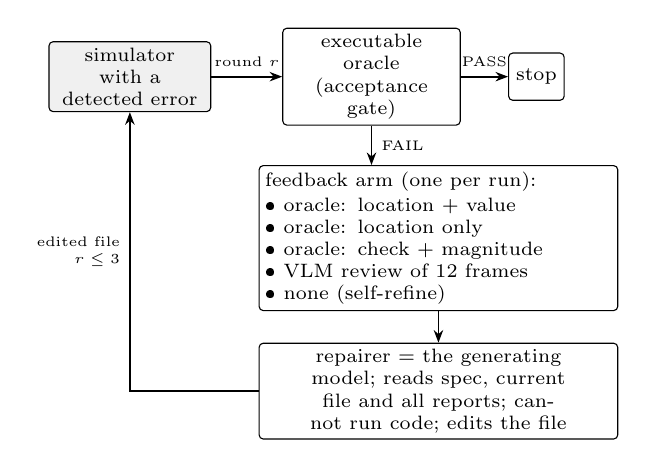
\begin{tikzpicture}[
  font=\scriptsize, node distance=4mm,
  box/.style={draw, rounded corners=1.5pt, align=center, inner sep=2.2pt, minimum height=6mm},
  data/.style={box, fill=black!6},
  arr/.style={-{Stealth[length=1.6mm]}, semithick}]
\node[data, text width=19mm] (file) {simulator with a detected error};
\node[box, right=9mm of file, text width=21mm] (oracle) {executable oracle\\ (acceptance gate)};
\node[box, right=6mm of oracle, text width=6mm, inner sep=1.5pt] (stop) {stop};
\node[box, below=5mm of oracle.south west, anchor=north west, xshift=-3mm, text width=44mm, align=left] (fb) {feedback arm (one per run):\\[1pt]
  \textbullet\ oracle: location + value\\
  \textbullet\ oracle: location only\\
  \textbullet\ oracle: check + magnitude\\
  \textbullet\ VLM review of 12 frames\\
  \textbullet\ none (self-refine)};
\node[box, below=4mm of fb, text width=44mm] (rep) {repairer = the generating model; reads spec, current file and all reports; cannot run code; edits the file};
\draw[arr] (file) -- node[above, font=\tiny]{round $r$} (oracle);
\draw[arr] (oracle) -- node[above, font=\tiny]{PASS} (stop);
\draw[arr] (oracle.south) -- node[right, font=\tiny]{FAIL} (oracle.south |- fb.north);
\draw[arr] (fb) -- (rep);
\draw[arr] (rep.west) -| node[pos=0.75, left, align=right, font=\tiny]{edited file\\ $r \le 3$} (file.south);
\end{tikzpicture}
\caption{Iterative repair. Oracle arms stop when the oracle passes; the VLM arm stops when the reviewer says ``correct'' and self-refinement when the repairer replies \texttt{NO\_CHANGE}. The oracle grades every arm's final file, but only the oracle arms see its verdict.}\label{fig:loop}
\end{figure}


\paragraph{Repair} Every simulator with an oracle-detectable natural error enters an iterative repair loop (Fig.~\ref{fig:loop}). The repairer is the model that generated the file. In each round it reads the specification, the current file and all feedback reports so far, edits the file in place and replies \texttt{CHANGED} or \texttt{NO\_CHANGE} with a one-line reason. It may not run code or read any other file. This isolates the information it receives through feedback, at the cost of disadvantaging self-refinement relative to an agent that can execute. Five feedback arms are compared:
\begin{itemize}
\item the three oracle levels of Section~\ref{sec:feedback} (\emph{spec}, \emph{locate}, \emph{coarse}), each stopping when the oracle passes;
\item \emph{VLM in the loop}: a fresh, blinded VLM review of the current version, stopping when the VLM says the simulator is correct;
\item \emph{self-refine}: a generic ``a reviewer suspects errors, re-check against the specification'' prompt, stopping when the repairer replies \texttt{NO\_CHANGE}.
\end{itemize}
All arms have a budget of $K=3$ rounds. Every version in every arm is graded by the oracle, whether or not the arm shows the grade to the repairer, so final correctness is measured the same way for all arms.

\subsection{Phases and repetitions}
The study evolved in phases, each motivated by the previous one. All data are reported.
\begin{enumerate}
\item Detailed specification, 4 mechanisms, 8 simulators and 24 mutants: no natural errors.
\item Spec-lite, 4 mechanisms (four-bar, Geneva, Jansen, planetary), 2 samples per cell.
\item One round of repair on the 7 faulty files with oracle, VLM or no feedback.
\item Iterative repair ($K=3$) on the same files.
\item The full design: cam and Watt six-bar added, 5 samples per cell (60 simulators), and iterative repair repeated twice. Repetition 1 covers the 8 newly faulty files; repetition 2 covers those 8 plus the 7 files of phases 2--4.
\item The \emph{locate} arm on exactly the file-runs of phase~5.
\item Chebyshev lambda and Peaucellier--Lipkin added (20 simulators) and iterative repair with the four non-VLM arms.
\end{enumerate}
Phases 3 and 4 shaped the design (they showed that one round is too little to separate the arms and that feedback must be localised), and we report them only briefly. The main repair analysis uses the 22 file-runs of phases 5--6 and the 6 of phase~7.

\subsection{Measures and statistics}
For RQ1 the unit is a generated simulator. Every oracle failure was inspected by hand to confirm that the error is real; Section~\ref{sec:results} also reports one error that the oracle cannot see. For RQ2 the unit is a simulator or mutant, and we report true and false positives of the oracle and the VLM. For RQ3 and RQ4 the unit is a \emph{file-run}, a faulty file in one repetition, and the outcome is whether its final version passes the oracle. All arms are applied to the same file-runs, so we compare them as paired binary outcomes: Cochran's $Q$ across arms, exact McNemar tests per pair with Holm correction, Wilson 95\% intervals for proportions, and Fisher's exact test between models. Repetition~2 contains the files of repetition~1, so file-runs are not fully independent. We therefore repeat the main tests with each source file counted once.

\subsection{Use of large language models}
Following the journal's policy, we state how LLMs were used. They are the \emph{object} of study: they generated, reviewed and repaired the simulators as described above. Claude Code (with \texttt{claude-opus-5-5}) was also used as a programming assistant to implement the oracle, the reference simulators, the mutants and the analysis scripts, under the author's direction. Every oracle failure on generated code was checked by hand, the reference simulators were verified numerically, and the statistics were spot-checked by hand calculation. The same assistant helped draft and edit the manuscript text and searched the related literature; the author checked every number against the data and every reference against its source, and takes full responsibility for the content.

\section{Results}\label{sec:results}

\subsection{RQ1: errors in generated simulators}\label{sec:rq1}

\paragraph{Detailed versus free-form specifications} With the detailed specification, which fixed coordinates, branches and formulas, all 8 generated simulators passed the oracle (0/8, Wilson 95\% CI 0--32\%). With the free-form description of the same kind of mechanism, errors appeared at once: 7 of the first 16 simulators were wrong (44\%, CI 23--67\%; Fisher's exact test against the detailed specification $p=0.054$). Once the model has to \emph{choose} the dimensions and the assembly, errors move from writing kinematics code to recalling and applying design knowledge.

\paragraph{Error rates per mechanism} Table~\ref{tab:natural} shows the 80 free-form simulators. Twenty fail the oracle: 13 of 40 by the smaller and 7 of 40 by the larger model. On the Jansen leg, 9 of 10 simulators were wrong; on Chebyshev's lambda linkage, 6 of 10. Elsewhere, only 5 of 60 were wrong (8\%).

% generated by make_tables.mjs from pilot/results/gen_lite5.jsonl and gen_lite7.jsonl -- do not edit by hand
\begin{table}[t]
\caption{Natural errors: simulators generated from the free-form specification that fail the oracle (5 samples per cell)}\label{tab:natural}
\begin{tabular}{@{}llcc@{}}
\toprule
Mechanism & Design knowledge checked & Haiku & Sonnet \\
\midrule
Four-bar crank-rocker & Grashof condition & 0/5 & 1/5 \\
Geneva drive & tangential pin entry & 0/5 & 0/5 \\
Planetary gear set & assembly condition & 2/5 & 0/5 \\
Disk cam, roller follower & motion law, pressure angle & 0/5 & 0/5 \\
Watt II six-bar & transmission angle & 1/5 & 1/5 \\
Jansen leg & published link lengths & 5/5 & 4/5 \\
Chebyshev lambda & published proportions & 5/5 & 1/5 \\
Peaucellier--Lipkin & geometric relations & 0/5 & 0/5 \\
\midrule
Total & & 13/40 & 7/40 \\
\botrule
\end{tabular}
\end{table}


\begin{figure}[!htbp]
\centering
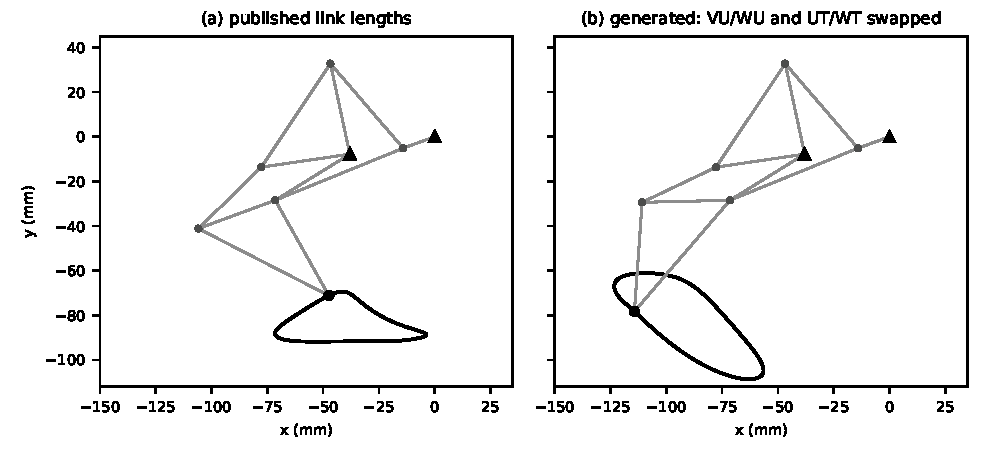
\includegraphics[width=0.82\textwidth]{figures/jansen.pdf}
\caption{Jansen leg solved from (a) the published link lengths and (b) the \texttt{SIM.params} of a simulator generated by the larger model, which swapped \texttt{VU}/\texttt{WU} and \texttt{UT}/\texttt{WT}. Grey: linkage at one crank angle; black curve: path of the foot T over one crank revolution; triangles: fixed pivots. Both pages run and animate without errors.}\label{fig:jansen}
\end{figure}

All 20 failures were confirmed by hand. They fall into four classes:
\begin{itemize}
\item \emph{Misremembered design knowledge} (15). In all nine faulty Jansen legs the generator recalled the published numbers but assigned some of them to the wrong links, or scrambled them, for example a crank of 38 instead of 15. Figure~\ref{fig:jansen} shows a leg with two swapped pairs: the page runs, animates and looks like a Strandbeest, but the foot no longer has a flat ground-contact segment. With the lengths of the first two faulty legs, the flat part of the foot path shrank from 36\% to 6\% of the cycle and the stride from 49 to 11~mm. All five lambda linkages from the smaller model used ordinary four-bar proportions instead of Chebyshev's, and the larger model once placed the tracing point at the middle of the coupler instead of its extended end. A direct check of path straightness agrees with the proportion check on all ten lambda simulators: the four that pass trace a near-straight segment (1\% of the crank length) over $200^\circ$, and the six that fail have no such segment. No correct alternative design was rejected.
\item \emph{Violated assembly conditions} (4). Two planetary sets had $Z_s+Z_r=100$, not divisible by three, so three equally spaced planets cannot mesh with both sun and ring. Two Watt six-bars had a second loop that cannot close for part of the cycle.
\item \emph{Runtime failure} (1). A four-bar threw an exception on load because it assigned to a read-only property.
\item \emph{Geometry outside the contract} (1, not in the table). In one Geneva drive the cut-out of the locking disc faced away from the pin, so the wheel is not locked during dwell and the disc overlaps the wheel during indexing. The oracle cannot see this, because it checks markers, not the outline of the drawn parts; the VLM reviewer found it (Section~\ref{sec:rq2}).
\end{itemize}
Mechanisms whose design rule is a relation that the description implies produced no errors at all. This holds for the cam (0/10), whose motion law the description states, and for the Peaucellier--Lipkin linkage (0/10), whose conditions the models stated correctly in every case. The difference between models is clearest on the lambda linkage: 5/5 wrong for the smaller model versus 1/5 for the larger ($p=0.048$).

\paragraph{Another vendor} The two DeepSeek models of phase~8 show the same pattern on the two design-knowledge mechanisms. One of the 20 replies was cut off at the output limit and contained no page, so 19 simulators ran. The larger model was wrong on 9 of 10 (Jansen 5/5, lambda 4/5) and the smaller on 5 of 9 (Jansen 4/4, lambda 1/5). Every failure was a DESIGN failure of the proportion check, and inspection confirmed each one. As with Claude, the Jansen legs used the published numbers but assigned some of them to the wrong links. None of the five faulty lambda linkages had Chebyshev's proportions. Here the relation between models is reversed: the larger DeepSeek model erred more often on lambda than the smaller. Error rates on recalled design knowledge are therefore high across vendors, but which model is worse is not stable.

\subsection{RQ2: what the oracle and the VLM detect}\label{sec:rq2}

\paragraph{Seeded mutants} The oracle detected all 24 detailed-specification mutants, all 15 spec-lite mutants, and, with the drift check, the gamed mutant. On the 24 detailed-specification mutants, checks that need no ground truth (META and structural checks) already caught 17: all state, length and phase faults, three of four branch faults and two of four direction faults. The remaining seven, a four-bar on the crossed branch, two reversed directions and four panel faults, need the kinematic solution. The VLM reviewer detected 20 of 24 mutants when the numeric panel was visible and 14 of 24 without it. Its detection of 10--15\% length errors fell from 4/4 to 1/4. From its explanations, the VLM recovered lengths mainly by reading the panel and solving the kinematics itself, not by inspecting the drawing. Paired by mutant, the oracle's advantage is significant against the VLM without panel (10 versus 0 discordant mutants, exact McNemar $p=0.002$) but not against the VLM with panel (4 versus 0, $p=0.125$). Among the four mutants the VLM missed with the panel visible, it saw a $12$--$20^\circ$ slot offset of the Geneva wheel but attributed it to perspective.

\paragraph{Natural errors} On the 15 renderable simulators of phase~2, the VLM found 5 of the 6 oracle-detected errors and reported 1 false positive on 9 correct simulators. It missed the planetary assembly violation, which is invisible in a rendering, but found the Geneva disc error that the oracle cannot see. On the 44 new simulators of phase~5 it had 7 true positives, 1 false negative (again a planetary tooth-count violation) and 4 false positives, all Geneva drives. The marker data show these wheels index by exactly $72^\circ$ per driver turn; the reviewer misread intermittent motion as a fault. The VLM was also unstable: a fresh review of the same unchanged files at the start of repetition~2 called three faulty simulators correct, among them the Geneva drive it had flagged before.

The two oracles are complementary. The executable oracle catches errors of design knowledge and invisible errors (assembly conditions, state, panel values) deterministically, in about 0.2~s and with no model calls. The VLM catches shape errors outside the marker contract but misses invisible ones, produces false alarms on intermittent motion, and costs about 52{,}000 tokens per review.

\subsection{RQ3: the oracle as an acceptance gate for repair}\label{sec:rq3}

In two preliminary phases, one round of repair fixed 3 of 7 faulty files whether the feedback came from the oracle (as check names and magnitudes), the VLM or nobody. With three rounds, specific oracle feedback fixed 6 of 6 against 4/6 (coarse oracle), 2/6 (VLM) and 0/6 (self-refine). Tables~\ref{tab:rounds} and~\ref{tab:repair} report the full design.

% generated by make_tables.mjs from pilot/iter5/*/summary.json -- do not edit by hand
\begin{table}[!htbp]
\caption{File-runs passing the oracle after each repair round, phases 5--6 pooled (22 file-runs; round 0 = generated file)}\label{tab:rounds}
\begin{tabular}{@{}lcccc@{}}
\toprule
Arm & r0 & r1 & r2 & r3 \\
\midrule
location + value & 0 & 16 & 22 & 22 \\
location only & 0 & 12 & 14 & 14 \\
check + magnitude & 0 & 8 & 10 & 10 \\
VLM review in the loop & 0 & 5 & 5 & 5 \\
Self-refine (no feedback) & 0 & 6 & 6 & 6 \\
\botrule
\end{tabular}
\end{table}

% generated by make_tables.mjs from pilot/stats/stats.json -- do not edit by hand
\begin{table*}[t]
\caption{Iterative repair (at most three rounds): file-runs whose simulator passes the oracle at the end, by feedback arm. Assembly/constraint errors: Watt six-bar, planetary, four-bar crash. Design knowledge: Jansen (phases 5--6) and Chebyshev lambda (phase 7). The VLM arm was not run for the lambda file-runs (n/a).}\label{tab:repair}
\begin{tabular}{@{}lcccc@{}}
\toprule
Feedback arm & Assembly / constraint & Design knowledge, Haiku & Design knowledge, Sonnet & All \\
\midrule
Oracle, location + value & 8/8 & 13/13 & 7/7 & 28/28 \\
Oracle, location only & 8/8 & 0/13 & 7/7 & 15/28 \\
Oracle, check + magnitude & 8/8 & 0/13 & 3/7 & 11/28 \\
VLM review in the loop & 5/8 & 0/8\textsuperscript{a} & 0/6\textsuperscript{a} & 5/22\textsuperscript{a} \\
Self-refine (no feedback) & 6/8 & 0/13 & 1/7 & 7/28 \\
\botrule
\end{tabular}
\footnotetext[a]{Lambda file-runs excluded (no VLM arm).}
\end{table*}


Over the 22 file-runs of phases 5--6, feedback with location and correct value fixed all 22, all within two rounds. It was followed by location only (14), check and magnitude (10), self-refinement (6) and VLM in the loop (5). The arms differ (Cochran's $Q=44.5$, $df=4$, $p=5\times10^{-9}$). After Holm correction, full oracle feedback beats every other arm (location only $p=0.047$, coarse $p=0.004$, VLM $p=1.5\times10^{-4}$, self-refine $p=2.7\times10^{-4}$), and location-only beats VLM ($p=0.027$) and self-refinement ($p=0.047$). Location-only versus coarse (4 versus 0 discordant file-runs) and coarse versus VLM or self-refinement are not significant. With each source file counted once (20 file-runs including lambda, four arms) the conclusions do not change: full feedback 20/20 versus location only 10/20 (Holm $p=0.008$), coarse 8/20 ($p=0.002$) and self-refinement 4/20 ($p=1.8\times10^{-4}$).

The difficulty splits by error class. Assembly and runtime errors were repaired with any oracle feedback (8/8 in all three oracle arms) and often even without (self-refinement 6/8, VLM 5/8); the arms do not differ significantly on this class ($Q$ test $p=0.064$). Design-knowledge errors were repaired almost only with oracle feedback, as RQ4 details.

The two loops without an executable gate failed in characteristic ways. VLM-driven loops stopped 12 times on a ``correct'' verdict while the oracle still failed the file, and the VLM never recognised the planetary tooth-count error, so its arm did worse than self-refinement even on assembly errors. Self-refinement stopped when the repairer answered \texttt{NO\_CHANGE}, and all 17 such answers on faulty Jansen legs declared the file correct; 10 of them stated explicitly that the link lengths ``match Jansen's holy numbers''. In one case the repairer stated that nothing was wrong with a four-bar that did not load.

\paragraph{Is a repairer needed at all?} Because the full report states the correct values, we also ran a deterministic baseline without any model. It takes the values that the location + value report on the original file gives as ``expected'' and writes them into the page. Two variants were tried:
\begin{itemize}
\item \emph{Patching \texttt{SIM.params} at load time}: 0 of 28 file-runs passed (20 source files). The design check then passed, but every page had built its link geometry from the old lengths, so the drawing no longer matched the parameters.
\item \emph{Rewriting the numeric literals in the page source}, the more favourable variant, so that the geometry is built from the corrected values: 11 of 28 file-runs passed (9 of 20 source files; Table~\ref{tab:repair}).
\end{itemize}
The patch cannot touch assembly, tooth-count or runtime errors, for which the report names a violated condition but no value (0/8). On design-knowledge errors it fixed 11 of 20. The other nine still failed for three reasons. With the corrected lengths, some pages solved the linkage on a different assembly branch. In others, parts no longer met at shared joints. In the rest, a frame marker or the tracing point was drawn by separate code that the patch did not reach. The model given the same report fixed all 28. The LLM is therefore not a transcriber of numbers. It keeps the code, the drawing and the panel consistent with the corrected design, and it repairs faults for which no value exists.

\subsection{RQ4: how specific must feedback be?}\label{sec:rq4}

Pooling the design-knowledge file-runs (Jansen, phases 5--6, and lambda, phase 7), the result depends strongly on the repairing model (Table~\ref{tab:repair}):
\begin{itemize}
\item The smaller model fixed 13 of 13 with location and value and 0 of 13 with location only, coarse feedback or no feedback (Cochran's $Q=39$, $p=1.7\times10^{-8}$; each pair with the full arm exact McNemar $p=2.4\times10^{-4}$, Holm $p=0.001$; counting each source file once, 10/10 versus 0/10, Holm $p=0.012$).
\item The larger model fixed 7 of 7 with location and value \emph{and} 7 of 7 with location only, 3 of 7 with coarse feedback and 1 of 7 without feedback.
\item With location only, the two models differ sharply (7/7 versus 0/13, Fisher $p=1.3\times10^{-5}$); with location and value they do not (7/7 versus 13/13, $p=1$).
\end{itemize}
The lambda linkage, added to test whether this pattern was specific to Jansen, reproduced it. The smaller model fixed 5/5 with values and 0/5 in each of the three other arms; the larger model's single faulty file was fixed in every arm, including self-refinement.

The repairers' replies show why location is not enough for the smaller model. The ``looks swapped with'' hints let it undo permutations. In two lambda files this left a single wrong link, the distance to the tracing point, which has to be recalled (five crank lengths). It never recovered that value in three rounds. Instead it substituted other proportions it believed to be classical (several different sets across files and rounds, none correct), back-computed a length from the reported error magnitude (four attempts, all wrong, since the minimax formula is not in the feedback), or answered \texttt{NO\_CHANGE}. On Jansen, 9 of the 40 location-only attempts were \texttt{NO\_CHANGE} replies claiming that the lengths matched the published numbers and that the checker's mapping must be wrong. The larger model, given only the names of the wrong links, supplied the published values from memory. With coarse feedback, it twice inferred the wrong Jansen link from the error magnitude itself, the only route by which coarse feedback fixed a Jansen leg.

\subsection{Reliability of the oracle}\label{sec:reliability}
The reference simulators pass, and every seeded mutant is detected. Every oracle failure on a generated simulator was confirmed by hand, so we observed no false positives. The single false negative is the Geneva disc of Section~\ref{sec:rq1}, which lies outside the contract. To exclude passes obtained by moving markers instead of parts, we audited all passing generated simulators and all passing final repaired versions, 146 files, for marker drift: all had a drift of zero. One repairer explicitly tried this tactic, saying it had set markers ``directly from the solved points'', but its version still failed the design check. After we added the drift check and changed the Jansen scale estimate, we regraded all 661 earlier verdicts. 660 were unchanged, and the gamed mutant moved from pass to fail. Rule violations by agents were rare. One of 155 phase-5 repair attempts ran a Python command despite the instruction, and one phase-7 attempt stopped without writing a reply, asking instead to be told the classical proportions.

\section{Discussion}\label{sec:discussion}

\paragraph{An executable gate, not a replacement for review} The oracle and the VLM catch different errors (RQ2). The oracle is deterministic, explains its verdicts and costs nothing per run, but it only sees what the contract exposes. The VLM sees the drawn shapes but cannot see invisible conditions, misreads intermittent motion, and changes its verdict between identical runs. In a generation pipeline we would therefore use the oracle as the \emph{acceptance gate} and repair driver, and keep a visual review as an additional, advisory check for shape errors outside the contract. In V\&V terms, this puts analytic comparison first and animation second \cite{sargent2013vv}. Our data show that a VLM alone as gate is not safe: 12 of its stop decisions accepted simulators that the oracle rejected.

\paragraph{Feedback should carry the reference value when one exists} Iterative repair with test feedback is well established \cite{chen2023selfdebug,xia2024chatrepair,olausson2024selfrepair}, and the quality of feedback is known to limit self-repair \cite{olausson2024selfrepair}. Our ablation isolates one dimension of that quality, \emph{information content}, at fixed source and wording, and shows that its effect depends on the model. Localisation alone sufficed for the larger model, which held the missing design knowledge, but did nothing for the smaller model, which did not. For a mechanism with published dimensions the oracle knows the correct value anyway, so withholding it has no benefit. More generally, an oracle that encodes reference knowledge should return that knowledge in its diagnostics, because the cheapest repairer may need it. This contrasts with feedback designs that report only failing tests or error magnitudes, and with results suggesting that weaker models mainly benefit from more feedback \cite{han2025convcodeworld,pan2025gfr}. In our setting it was the \emph{kind} of information that mattered, not its amount.

\paragraph{Confident wrong knowledge} The most consistent failure we saw was not an inability to edit code. It was a repairer that defended a wrong design with a confident and specific claim (``the lengths match the published holy numbers''), sometimes blaming the checker. Self-correction without external feedback is known to be unreliable \cite{huang2024cannot,kamoi2024selfcorrection}, and LLMs hallucinate domain facts in code \cite{liu2026codehallucination,tian2025codehalu}. Our data add that in an engineering domain such claims are cheap to falsify mechanically, but only if the acceptance step does not depend on the same model's judgement.

\paragraph{When is an oracle worth writing?} The oracle needed one module per mechanism type (27--90 lines of JavaScript each), written once and reused for every generated instance regardless of its dimensions. The checks that need no ground truth (META) already caught most seeded faults (17 of 24), and they transfer to any simulator that follows the contract. Errors were concentrated where design knowledge must be recalled rather than derived. Mechanisms specified by a relation or law that the description implies (cam, Peaucellier--Lipkin) produced no natural errors, whereas mechanisms that depend on remembered numbers (Jansen, lambda) produced most of them. A practical heuristic follows: invest in DESIGN rules for mechanisms whose function depends on published dimensions, and rely on the generic META, PARAM and GT checks elsewhere.

\paragraph{Leakage through magnitudes} Our coarse and location-only arms still reported the measured value of each failed check. The smaller model repeatedly tried to invert this value into a corrected length, without success because the minimax formula was not shown. The larger model succeeded twice on Jansen. Error magnitudes are thus a side channel between feedback levels, and future ablations should control them explicitly.

\section{Threats to validity}\label{sec:threats}

\paragraph{Construct validity} Correctness is defined by our oracle and by hand inspection by the author. The DESIGN rules encode engineering knowledge that we wrote. We verified the reference designs numerically (Jansen's foot path, the lambda straight segment, the Peaucellier line), but the rule set has not yet been reviewed by an independent mechanical engineer \todo{expert review}. The marker contract is a precondition of the oracle and may change how models write simulators. Errors outside the contract, such as the Geneva disc, are invisible to it, so ``passes the oracle'' does not mean ``correct'' in every respect. The feedback levels are produced by transforming the oracle's text. Location-only and coarse feedback still contain the measured magnitude of each failed check, which a repairer can partly exploit (Section~\ref{sec:discussion}).

\paragraph{Internal validity} Repairers were not allowed to run code, so that all arms received information only through feedback. Self-refinement by an agent that can execute its own page might do better. Agents ran as sub-agents of Claude Code with that tool's system prompt, not as raw model calls. One of 155 phase-5 repair attempts ran a command despite the instruction; we kept it in the data. The design evolved over phases (Section~\ref{sec:design}), and the feedback levels were introduced after seeing phase-4 results. To limit the resulting risk of tailoring, phases 6 and 7 re-used the exact file-runs and stopping rules of phase~5 and added mechanisms chosen \emph{before} their generations were seen.

\paragraph{External validity} Only two models of one vendor were used; a model from another vendor is the most important missing replication \todo{other-vendor model}. The mechanisms are planar, single-input and textbook-sized. The significant RQ4 effect rests on two mechanisms with published dimensions (Jansen and lambda). The relation-type mechanism (Peaucellier--Lipkin) produced no natural errors, so it could not be tested on real faults. Simulators followed a reduced contract derived from one generation tool.

\paragraph{Conclusion validity} Samples are small (22 + 6 file-runs for repair). Repetition~2 contains the files of repetition~1, so file-runs are not independent. We report exact tests, Holm-corrected pairwise comparisons and an analysis that counts each source file once; the main effects (full oracle feedback versus all other arms; the model $\times$ feedback interaction) remain significant under it. Several pairwise differences, such as location-only versus coarse and oracle versus VLM with panel on mutants, are not significant, and we do not claim them.

\section{Related work}\label{sec:related}

\paragraph{LLM-generated 3D and physics code} Benchmarks for interactive scientific demonstrations \citep{chen2025interactscience}, physics animations \citep{wang2026simuscene}, physics-aware 3D scenes \citep{xie2026physcodebench} and 3D worlds \citep{lu2026worldcoder} show that generated programs usually run but often behave wrongly. WorldCoder-Bench also finds that screenshot-based VLM judging correlates poorly with state-level correctness. Generators of articulated objects and CAD models use a VLM critic in the loop \citep{gao2026lam,le2025articulate,alrashedy2025cad}, as does agentic generation of physics simulation code \citep{shende2026perceptual}, which names the remaining ``oracle gap''. SGA verifies educational animations through their scene graph \citep{lopez2026sga}. Closest in domain are LLM-based linkage synthesis \citep{gandarela2025msynth,gandarela2026linkage}, where a trusted simulator evaluates parameters the LLM proposes, and the generation of multibody models compared with expert ground truth \citep{gerstmayr2026meceng}. In contrast, we test the simulator code itself, derive the ground truth from the simulator's declared parameters, and study the oracle as gate and feedback source.

\paragraph{Test oracles and metamorphic testing} Our oracle is a derived oracle in the sense of \citet{barr2015oracle}. Its META family consists of metamorphic and structural relations \citep{chen2018metamorphic,segura2016survey} implied by the output contract, analogous to metamorphic testing of graphics compilers \citep{donaldson2017shader}, scientific software \citep{kanewala2014scientific} and autonomous-driving systems \citep{zhou2019driverless}. Work on oracle automation with neural models \citep{dinella2022toga,hossain2023neural,molina2025oracle} generates assertions. We instead encode reusable domain rules once per mechanism type and keep the oracle independent of the model under test, as recommended by \citet{molina2025oracle}. Insufficient tests over-accept LLM code \citep{liu2023evalplus}, and property-based tests have been proposed as a remedy \citep{vikram2023pbt}; our setting has no tests at all, so the oracle has to provide them.

\paragraph{Simulation V\&V} Classical simulation V\&V lists both animation and comparison with analytic results among validation techniques \citep{sargent2013vv,balci1997vva,kleijnen1995vv}. Our comparison of VLM review and executable oracle can be read as a comparison of these two techniques, automated, for generated simulators.

\paragraph{Repair with feedback} Self-Debug \citep{chen2023selfdebug}, Reflexion \citep{shinn2023reflexion} and Self-Refine \citep{madaan2023selfrefine} use execution or self-generated feedback. \citet{olausson2024selfrepair} show that feedback quality limits self-repair. Without an external signal, self-correction is unreliable \citep{huang2024cannot,kamoi2024selfcorrection}. Among SE approaches, ChatRepair \citep{xia2024chatrepair} repairs in conversation with test-failure feedback until tests pass, and \citet{fan2023repairllm} repair LLM-generated programs and find location information useful. ConvCodeWorld \citep{han2025convcodeworld} varies the type and quality of feedback (compilation, execution with partial or full test coverage, novice or expert verbal feedback) in conversational code generation, and \citet{pan2025gfr} vary model strength in the generator, feedback and refiner roles. To our knowledge, no prior study uses a single deterministic oracle to deliver feedback at controlled levels of information (location with value, location only, check with magnitude), compares them with VLM review and self-refinement under oracle-gated stopping, and reports an interaction between the needed information and the repairing model.

\paragraph{LLM and VLM judges} LLM judges are biased and unreliable for code correctness \citep{zheng2023judging,wang2024notfair,crupi2025llmjudgecode}, and multimodal judges and VLMs struggle with simple geometry and visual glitches \citep{chen2024mllmjudge,rahmanzadehgervi2024blind,taesiri2024glitchbench}. Our VLM results (unstable verdicts, false alarms on intermittent motion, invisible conditions missed) are consistent with this literature in a new domain.

\paragraph{Models, simulations and AI in systems engineering} Related systems-engineering work checks that a rendered block diagram matches its model \citep{waldvogel2026blockdiagram}, classifies AI for software engineering \citep{schieferdecker2026ai4se} and uses LLMs to interpret test logs of a digital twin \citep{hermawan2026log}. We are not aware of work on executable oracles for LLM-generated simulation code.

\section{Conclusion}\label{sec:conclusion}

Generated mechanism simulators run and look right much more often than they are right. Under free-form specifications, a quarter of the simulators in our study were wrong, mostly in design knowledge that the model had to recall. An executable oracle that derives its ground truth from the simulator's own declared parameters, plus a small set of design rules per mechanism type, detected these errors deterministically at negligible cost. Used as the acceptance gate of an iterative repair loop with diagnostics that name the faulty element and its correct value, it led to correct simulators in every faulty case within two rounds. VLM review and self-refinement stopped on wrong ``correct'' verdicts. How much the feedback must say depends on the repairing model: a larger model needed only the location of the error, a smaller one the correct value.

Future work includes replication with models from other vendors, mechanisms beyond planar linkages, contracts that expose part outlines so that shape errors become checkable, generating DESIGN rules from engineering references, and controlling the magnitude side channel in feedback ablations.


%% ISSE requires a "Statements and Declarations" section; Author Contribution and Competing Interest must also be
%% entered in the submission system. Fill in the TODOs before submission.
\section*{Statements and Declarations}

\bmhead{Funding} \todo{funding statement, or: ``No funding was received for conducting this study.''}

\bmhead{Competing interests} The author has no relevant financial or non-financial interests to disclose.

\bmhead{Ethics approval} Not applicable; the study involves no human participants or personal data.

\bmhead{Data and code availability} The specifications, generated and repaired simulators, mutants, reference simulators, oracle, feedback texts, repair replies, raw oracle results and analysis scripts are available at \url{https://github.com/haihpse150218/llm-mechsim-oracle} and archived at \todo{Zenodo DOI}. The repository README explains how to regenerate every table and statistic in this paper (\texttt{pilot/stats/stats.mjs}, \texttt{paper/draft/make\_tables.mjs}).

\bmhead{Author contributions} Phi Hai Hoang is the sole author and was responsible for conceptualisation, methodology, software, validation, formal analysis, investigation, data curation, visualisation, and writing (original draft, review and editing).

\bmhead{Use of generative AI} See Section~\ref{sec:design}, ``Use of large language models''.


\bibliography{../references,llm3d}

\end{document}
